\documentclass[10pt,amsmath,twocolumn,aps,prl,superscriptaddress,floatfix]{revtex4-1}
%\documentclass[journal=jacsat,manuscript=article]{achemso}
\usepackage{epsfig,color,graphicx,amsmath,chemformula,xr}
\usepackage[T1]{fontenc}

\newcommand{\Ang}{\ensuremath{\mathring{\text{A}}}}
\newcommand{\ltwid}{\mathrel{\raise.3ex\hbox{$<$\kern-.75em\lower1ex\hbox{$\sim$}}}}
\newcommand{\gtwid}{\mathrel{\raise.3ex\hbox{$>$\kern-.75em\lower1ex\hbox{$\sim$}}}}
\newcommand{\bra}{\langle}
\newcommand{\ket}{\rangle}
%\newcommand{\sill}{\psi_\mathrm{SILL}}
\newcommand{\sill}{\psi}
\newcommand{\trace}{{\rm Tr}}
\newcommand{\ntilde}{\tilde{n}}
\newcommand{\stilde}{\tilde{s}}
\newcommand{\atilde}{\tilde{\alpha}}
\newcommand{\new}{\color{red}}
\newcommand{\blue}{\color{blue}}
\newcommand{\old}{\color{black}}
\newcommand{\bea}{\begin{eqnarray}}
\newcommand{\eea}{\end{eqnarray}}
\newcommand*{\MAINTEXT}{}
\def\nn{\nonumber\\}

%\bibliographystyle{naturemag}
\externaldocument[ext1-]{covalency_SI}


\begin{document}

\title{
\ifdefined\MAINTEXT
\else
Supplementary Information: \\
\fi
Contribution of the covalent component of the hydrogen-bond network to the properties of liquid water
}

\author{Yifei Shi}
\affiliation{Department of Chemistry, McGill University, 801 Sherbrooke St. West, Montreal, QC H3A 0B8, Canada}
\author{Hayden Scheiber}
\affiliation{Department of Chemistry, McGill University, 801 Sherbrooke St. West, Montreal, QC H3A 0B8, Canada}
\author{Rustam Z. Khaliullin}
\email{rustam.khaliullin@mcgill.ca}
\affiliation{Department of Chemistry, McGill University, 801 Sherbrooke St. West, Montreal, QC H3A 0B8, Canada}




%\begin{tocentry}
%\begin{center}
%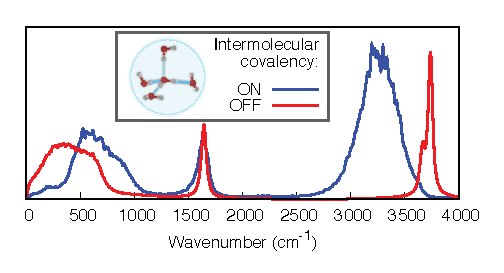
\includegraphics[height=3.5cm]{TOC/TOC}
%\end{center}
%\end{tocentry}

% RZK: format references as needed, Thomas Kuehne name is spelled incorrectly in several references
\ifdefined\MAINTEXT
\begin{abstract}
Many remarkable properties of liquid water originate from the ability of its molecules to form hydrogen bonds, each of which emerges as a combination of electrostatic, polarization, dispersion, and donor-acceptor or covalent interactions.
In this work, \emph{ab initio} molecular dynamics was tailored to isolate and switch off the covalent component of interactions between water molecules in simulations. 
Comparison of simulations with and without covalency shows that a small amount of intermolecular electron density transfer has a profound effect on the structure and dynamics of the hydrogen-bond network and thus on observable properties of room-temperature liquid water. 
%The findings of this study do not only deepen our knowledge about the fundamental nature of hydrogen bonding, but can also aid interpretation of spectroscopic response, catalytic behavior, and solvation properties of aqueous systems.
\end{abstract}

\maketitle


\section{Introduction} 

Detailed understanding of the physical nature of hydrogen bonding (HB) between molecules in water is essential for unraveling the origins of the unique physical and chemical properties of this ubiquitous and important liquid. 
Since the dawn of quantum mechanics, it has been known that HB is a complex phenomenon that arises from the interplay of several distinct effects: interaction between molecules' permanent multipoles (dipoles, quadrupoles, etc.), polarization, dispersion, and orbital donor-acceptor interactions~\cite{eisenberg2005structure}.

Donor-acceptor interaction leads to the transfer of electron density between molecules and is therefore known as the charge-transfer or covalent component of HB. 
The concept of intermolecular covalency, described canonically as lone electron pairs of oxygen atoms donated to nearby hydrogens, has been tremendously useful to describe physics and chemistry of water and is deeply embedded into the everyday chemistry language. 
It helps explain water's unique properties as a solvent and its ability to catalyze a wide variety of chemical processes. Covalent interactions can also explain the strong cooperativity between hydrogen bonds in systems ranging from nanodroplets to solvated biomolecules. 
From a theoretical standpoint, the covalent component of HB has attracted significant attention because of its purely quantum mechanical nature, which---unlike electrostatic and dispersion interactions---is difficult to describe with simple analytical force-field models~\cite{lee2011effects, gordon2013accurate}.

Recent developments in energy decomposition techniques based on accurate electronic structure methods have helped make substantial progress towards quantifying the individual contributions of various physical effects to the HB binding energy in water clusters~\cite{stevens1987frozen, stone1993computation, chen1996energy, schenter1996natural, glendening2005natural, weinhold2005resonance, piquemal2005csov, khaliullin2009electron, cobar2012examination, guevara2016hydrogen}. 

The extent of intermolecular charge transfer in HB has remained the last unresolved issue until recently~\cite{isaacs1999covalency, ghanty2000hydrogen, stone2017natural}. 
Natural bond orbital analysis~\cite{weinhold1998natural} and natural energy decomposition analysis \cite{glendening1994natural} have suggested that charge transfer is the major component of HB~\cite{schenter1996natural,glendening2005natural,weinhold2005resonance} because---when charge transfer is neglected---these methods yield no binding at the water-dimer equilibrium geometry. 
After a debate spanning several decades, it has been argued that natural bond orbital analysis is not optimal for weak interactions~\cite{stone2017natural}. 
It appears that the covalent component of HB is better described by early decomposition methods~\cite{kitaura1976new, bagus1984new, bagus1992decomposition, stevens1987frozen, chen1996energy, stone1993computation} as well as their modern variants~\cite{mo2000energy, misquitta2013charge, khaliullin2007unravelling}. 
According to these methods, charge transfer contributes only around 20--30\% of the overall binding energy between water molecules in small clusters \cite{stevens1987frozen, stone1993computation, chen1996energy, piquemal2005csov, khaliullin2009electron, cobar2012examination}, in agreement with many chemists' long-held intuitive view of HB.

While energy decomposition methods have helped understand the importance of charge-transfer in the binding strength of gas-phase water clusters, nothing is known about the contribution of the covalent component of the HB network to the \emph{observed} properties of liquid water. 
A deep connection between the covalent interactions and features of the X-ray absorption~\cite{fransson2016x, NatureComm2013}, infrared~\cite{JPCL2013, Faraday2011, lenz2006theoretical}, and nuclear magnetic resonance~\cite{NatureComm2015} spectra of liquid water and small water clusters has been pointed out in several recent articles. 

In this work, we extended a recently developed energy decomposition method for periodic systems~\cite{Khaliullin2013JCTC} to perform an unprecedented \emph{ab initio} molecular dynamics study that estimates the contribution of the covalent component of HB to the structural, dynamical, and spectroscopic properties of liquid water at ambient conditions. 
Our results show that the seemingly insignificant covalent component of HB is defining for many properties of liquid water. 

\section{Methodology}

% Discuss how appropriate BLYP. It is extrememly important to emphasize the qulitative nature of this study. Admit that BLYP-D3 model does not capture the properties of water in perfect quantitative agreement and does benifit from some cancellation of errors but it is still OK to capture the drastic difference between the reference model and devalent model.

To estimate the influence of the covalent component of HB on the observed properties of liquid water, we compared the properties calculated with \emph{ab initio} molecular dynamics (AIMD) using two different models. 
One model incorporates the intermolecular covalency fully whereas the other removes it completely.

The first model is the conventional Kohn-Sham density functional theory (DFT) approach, in which the electrons of a water molecule are delocalized over all neighbors. 
This model is known to reproduce many properties of liquid water reliably, in semi-quantitative agreement with experimental measurements (see important comments below). 
In this work, the first model is referred to as the delocalized-electron or reference model. 

The second model is a constrained DFT method based on absolutely localized molecular orbitals (ALMO)~\cite{khaliullin2006efficient}. 
Unlike conventional DFT, ALMO DFT~\cite{Khaliullin2013JCTC} is able to confine each electron strictly to its own molecule and therefore completely remove the covalent component from intermolecular bonding. 
Mathematically, this is achieved by expanding Kohn-Sham molecular orbitals \emph{only} in terms of the atomic orbitals of the parent molecule~\cite{stoll1980use,khaliullin2006efficient, mo2000energy}.
Such molecular orbitals are called absolutely localized because they are localized on molecules, in the same sense as atomic orbitals are localized on atoms. 
In the interest of brevity, intermolecular interaction without covalent component will be referred to as \emph{devalent} interactions and the ALMO-based model will be called the localized-electron or the \emph{devalent} model. 
It is important to note that the devalent model retains all other physical effects, including the covalent component of \emph{intramolecular} OH bonds. %were variationally optimized on each AIMD each step to find the electronic ground state of the system.
Theoretical methods that ensure the covalent component of intermolecular bonding is removed accurately are described in Computational Methods, together with pertinent accuracy tests.

To keep electrons absolutely localized over the course of AIMD simulations, we extended the recently developed ALMO DFT method for condensed molecular systems~\cite{Khaliullin2013JCTC} so that the atomic forces can be computed analytically from the ALMO DFT energies (see Computational Methods).

All AIMD simulations---with either delocalized or localized molecular orbitals---were performed using the dispersion-corrected~\cite{grimme2010consistent} BLYP exchange-correlation functional~\cite{becke1988density, lee1988development} and the TZV2P basis set~\cite{vandevondele2007gaussian}. 
The temperature of simulations was set to 298~K. 
The size of the periodic cubic simulation box was fixed to reproduce the experimental 0.997~g$\cdot$cm$^{-3}$ density of ambient liquid water. 
Since removing intermolecular covalency can affect the density, we also performed a set of simulations for a system in which density was adjusted to 1~atm using constant pressure AIMD. 
The length of the AIMD simulations were chosen to obtain statistically meaningful results. 
A detailed description of the calculations is presented in Computational Methods.

\textbf{Accuracy of the reference model.} It is important to comment on the ability of the reference model to reproduce properties of real water. 
Unfortunately, the existing exchange-correlation functionals can reproduce properties of liquid water only in \emph{semi-quantitative} agreement with experimental measurements. 
Thus this work aims only at capturing major \emph{qualitative} changes in water properties induced by the elimination of the covalent component from intermolecular bonding. 

Like most generalized gradient approximation (GGA)~\cite{cheng2012alignment} and meta-GGA~\cite{chen2017ab} functionals, BLYP is known to underestimate the energy gap of water molecules~\cite{adriaanse2012aqueous}.
% ZZZ: any reviews of predicted water gaps?
% PNAS, 2017, 114 (41), 10846
% J. Phys. Chem. Lett., 2012, 3 (23), 3411.
Because of this, the strength of intermolecular binding is slightly overestimated and computed radial (angular) distribution functions have sharper peaks than those derived from X-ray (NMR) scattering experiments~\cite{gillan2016perspective, ma2012ab}.
% ma2012ab - JOURNAL OF CHEMICAL PHYSICS 137, 044506 (2012)
% gillan2016perspective: Gillan, Alfe, and Michaelides J. Chem. Phys. 144, 130901 (2016)
The overbinding effect also results in an underestimated diffusion constant~\cite{bankura2014structure}, overestimated viscosity~\cite{khaliullin2013microscopic}, and red-shifted peaks in the high-frequency region of the IR spectrum~\cite{lee2007dynamical}. 
Despite these imperfections, the magnitude of errors in the reference model is much smaller than the magnitude of changes induced by neglecting intermolecular covalency. 
This implies that the effects of covalency are large enough to be captured qualitatively with the chosen computational methods.

We note in passing that, to quantify the contribution of covalent interactions to the properties of liquid water precisely, it would be useful to perform molecular dynamics simulations using the forces obtained from constrained coupled-cluster wavefunctions. While coupled-cluster energy decomposition methods already exist~\cite{schneider2016decomposition,azar2012energy,azar2015similarity}, coupling them to a dynamical engine and performing simulations on sufficiently large length- and time-scales is difficult. Such simulations can be done in the future as a quantitative extension of the present work.
%Azar, R. Julian; Head-Gordon, Martin, JOURNAL OF CHEMICAL PHYSICS   Volume: 136   Issue: 2     Article Number: 024103
%Azar, R. Julian; Head-Gordon, Martin, JOURNAL OF CHEMICAL PHYSICS   Volume: 142   Issue: 20   Article Number: 204101

% We chose the traditional BLYP-D3 model to perform this study because its shortcomings are well documented. Despite improved accuracy in reproducing some properties of liquid water, there is no evidence that newer exchange-correlation functionals can provide significantly more reliable results for the specific task of our study. Moreover, the newer functionals are still semi-empirical in nature and are not guaranteed to be reliable for all properties of interest (e.g. energy gap). Until their performance is carefully examined the AIMD community might continue using - at least for a short while - traditional time-tested functionals like BLYP, the shortcomings of which are well-documented.

\section{Results and discussion}

The variational principle of quantum mechanics guarantees that removing covalent interactions weakens intermolecular bonding. 
ALMO-based decomposition energy analysis predicts that, in a water dimer, the transfer of 0.3\% of an electron contributes  7~kJ$\cdot$mol$^{-1}$ (37\%) to the overall stabilization of the hydrogen bond at equilibrium geometry, in agreement with earlier reports~\cite{stevens1987frozen,chen1996energy,piquemal2005csov,khaliullin2009electron}. This contribution is higher in the cooperative HB network of liquid water at ambient conditions: 1\% of an electron and 19 ~kJ$\cdot$mol$^{-1}$ per hydrogen bond, in agreement with a previous study \cite{kuhne2014nature}.

\textbf{Molecular structure.} The covalent component of weak intermolecular bonds has only a minor effect on the shape of water molecules. 
%The average length of intramolecular OH bonds changes from 0.992~\Ang\ in the reference model to 0.977~\Ang\ in the devalent model of water. 
%At the same time, the average intramolecular HOH angle changes from 105.5 degrees to 104.3 degrees, becoming closer to the value calculated for 298~K gas phase water molecules.
%
The average length of intramolecular OH bonds and the average intramolecular HOH angle decrease by less than 1.5\% when the intermolecular covalency is turned off, becoming closer to the average value calculated for 298~K gas phase water molecules. 
The effect of covalency on the structure of the HB network is far more pronounced. 
The oxygen-oxygen radial distribution function (RDF) in Figure~\ref{Fig:RDF}A shows that weaker devalent interactions lead to a considerable expansion in the first coordination shell of water molecules from the reference average of 2.8~\Ang\ to 3.1~\Ang. 
The shift of the first-shell peak is accompanied by broadening that is indicative of a wider variety of configurations available to devalent HBs.

\begin{figure}
\includegraphics[width=0.45\textwidth]{new_rdf}
\includegraphics[width=0.45\textwidth]{new_adf}
\caption{A. Oxygen-oxygen radial distribution function. The experimental curve is taken from Ref.~\citenum{skinner2013benchmark}. B. Distribution of HB angles $\phi \equiv O_{\text{ref}} \cdots O-H$ computed for hydrogens within 2.3~\Ang\ from a reference atom. The angular distribution function is normalized to account for the $\phi$-dependent volume and to correctly emphasize the energetic preference for linear HBs (see Supplementary Information). The experimental curve is taken from Ref.~\citenum{modig2003temperature}.} \label{Fig:RDF}
\end{figure}

These dramatic changes in the structure of the HB network are consistent with the decrease in HB strength. 
It is remarkable, however, that the remaining components of HB---permanent electrostatic, polarization, and dispersion interactions---are sufficiently strong to retain several characteristic structural features of the network, including well-defined coordination shells and directional HBs~\cite{arunan2011definition}. 
% arunan2011definition: author list is not complete
Indeed, the second coordination peak in the RDF of the devalent model remains clearly visible though shifted to higher distances. 
The distribution of HB angles also retains a maximum at 0$^\circ$ despite becoming significantly broader (Figure~\ref{Fig:RDF}B).

The structure of the HB network for both models can also be illustrated with the spatial distribution of oxygen atoms around a reference water molecule (see cross sections in Figure~\ref{Fig:SDF}). 
It is clear that the distorted tetrahedral structure of liquid water is retained without the covalent component (cf. Figure~\ref{Fig:SDF}A and \ref{Fig:SDF}B), indicating that permanent electrostatic and polarization interactions tend to orient water molecules the same way as covalent interactions. 
For comparison, HBs become truly non-directional with uniform angular distribution if a water model includes only the Lennard-Jones potential (Figure~\ref{Fig:SDF}C). %retains only dispersion interactions and short-distance repulsion,  
This is why permanent electrostatics is widely recognized as the key component of interaction between water molecules and is included in all analytical molecular mechanics models of water. 
On the other hand, the equally strong covalent component is neglected in these models and instead compensated for by fine-tuning permanent atomic charges (see, for example, the spatial distribution for TIP3P water in Figure~\ref{Fig:SDF}D). 

\begin{figure*}
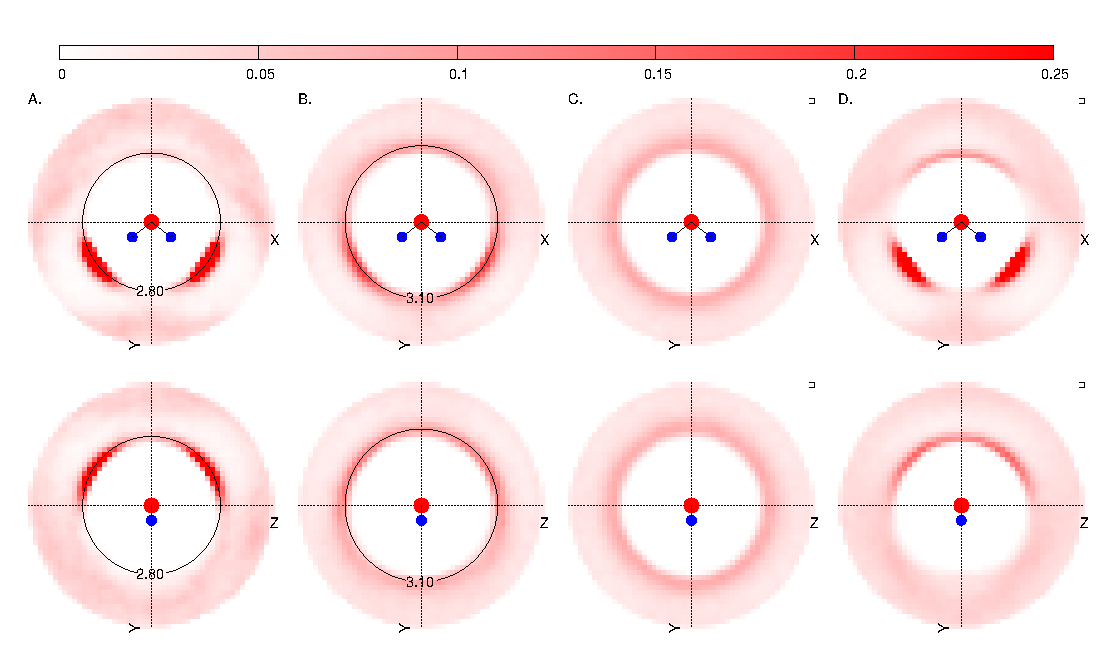
\includegraphics[width=0.9\textwidth]{SDF}
\caption{Cross sections of the spacial distribution of oxygen atoms. 
The upper panels show the cross section of the spacial distribution function in the plane of the reference water molecule, whereas the lower panels show the cross section in the plane bisecting the molecule. 
A. Reference model, B. devalent model, C. Lennard-Jones potential taken from TIP3P model, D. TIP3P model: electrostatic interactions combined with the Lennard-Jones potential~\cite{TIP3P}.} \label{Fig:SDF}
\end{figure*}
 
\textbf{HB statistics.} The drastic difference in the structure of the HB network of the reference and devalent models is confirmed by analysis of the HB statistics. 
The commonly accepted---though somewhat arbitrary---binary geometric definition of a HB is utilized: the H--O$\cdots$O angle must be smaller than 30$^{\circ}$ and the O-O distance must be shorter than 3.5\Ang~\cite{rey2002hydrogen,lawrence2003vibrational}. 
The distribution of molecules according to the number of donated or accepted HBs in Figure~\ref{fig:HBstat} shows that switching off intermolecular covalency leads to an increase of single-donor and single-acceptor molecules. 
The increase is so drastic that single-donor and single-acceptor molecules outnumber those with two HBs.
In total, the number of HBs in the devalent is reduced by approximately a third.

\begin{figure}
\includegraphics[width=0.45\textwidth]{new_hbstat}
%HOS: Increase text size to match figure 2?
\caption{HB statistics for liquid water with and without intermolecular covalency.}\label{fig:HBstat}
\end{figure}

\textbf{Density.} If the density is allowed to fluctuate in a simulation while the pressure is fixed at 1~atm, the average density decreases from 1.01~g$\cdot$cm$^{-3}$ for the reference model to 0.86~g$\cdot$cm$^{-3}$ for the devalent model, a decrease of 15\%. 
While this is a noticeable drop, it is important to note that the devalent water is still liquid at ambient conditions because of the strong electrostatic, polarization, and dispersion effects. 

The 15\% decrease in density would correspond to a 5\% increase in distances if all intermolecular bonds were stretched uniformly. 
However, intermolecular distances do not change uniformely with the size of the simulation box and the RDF of the devalent water remains largely unchanged if the density is allowed to relax (Figure~\ref{ext1-Fig:rdf_cp} in Supplementary Information). 
The only noticeable structural changes are the RDF peaks becoming slightly broader (Figure~\ref{ext1-Fig:rdf_cp}) and the angular distribution becoming narrower (Figure~\ref{ext1-Fig:ir_cp}) in the low-density constant-pressure model. 
This indicates that most molecules stay in the same position around the minimum of the potential well when the density is relaxed. 
Only a small fraction of them become distorted radially or angularly. 

In this work, we will continue discussing properties of the \emph{fixed-density} devalent water further because all key properties obtained for the \emph{fixed-pressure} model are almost the same, while performing fixed-pressure simulations is more time consuming (see Supplementary Information).

% density of butanol is 0.810, 3-Pentanone -- 0.815, 2-Octanol -- 0.824

\textbf{Infared spectrum.} Figure~\ref{Fig:IR} shows the infared (IR) spectra of the devalent and reference systems together with that of ideal water vapor at 298~K. The spectra are calculated entirely from the time-dependent positions of atoms and Wannier centers (Figure~\ref{Fig:acoord}) as described in Ref.~\citenum{thomas2013computing}.

\begin{figure}[ht]
\centering
\includegraphics[width=0.45\textwidth]{new_ir}
\caption{Calculated IR spectra. The far infrared part of the spectrum for the ideal-gas system, which corresponds to rotational modes, is removed for clarity. 
} \label{Fig:IR}
\end{figure}

\begin{figure}
\includegraphics[width=0.45\textwidth]{acoord}
\caption{Average positions of atoms (solid circles) and Wannier centers (empty circles) in a water molecule for the reference (black) and devalent (red) models. 
} \label{Fig:acoord}
\end{figure}

The most pronounced difference between the IR spectra is in the high-frequency region of intramolecular O--H stretching band $\nu_s$. 
%
It is important to note that it is extremely difficult to reproduce the high-frequency region of the IR spectrum of liquid water in quantitative agreement with experiment even by taking into account nuclear quantum effects~\cite{marsalek2017quantum} and by describing electrons with hybrid functionals or correlated wavefunction methods~\cite{medders2015infrared}. 
% medders2015infrared: J. Chem. Theory Comput., 2015, 11, 1145
% marsalek2017quantum: J. Phys. Chem. Lett., 2017, 8, 1545
However, several interesting qualitative conclusions can be drawn from the models employed in this work, without resorting to quantitatively accurate calculations. 
% we acknowledge that the agreement between our the reference simulations and experiment might be partially due to a cancellation of errors: the neglect of nuclear quantum effects can compensate deficiencies of the XC functional. Figure 3 in Ref.~\cite{marsalek2017quantum} suggests that the magnitude of the compensated error is only around 100 cm-1 and, importantly, its sign does not change our conclusions. 

For the reference liquid model, the $\nu_s$ peak is redshifted relative to that of gas-phase molecules -- a typical feature of hydrogen-bonded O--H groups.
At the same time, comparison of the spectra of the devalent and gas-phase models shows that the redshift disappears completely. 
This observation indicates that this feature of $\nu_s$ peak is entirely due to the covalent component of intermolecular interactions. 
Apparently, even the small amount of electron density transferred to the antibonding orbitals of intramolecular O--H bonds (see Figure~2 in Ref.~\citenum{khaliullin2009electron}) is sufficient to ``soften'' an intramolecular O--H bond---that is, decrease its force constant---and lower its vibrational frequency. 

The primary role of the covalent component in the broadening of the $\nu_s$ peak is also apparent from Figure~\ref{Fig:IR}. 
The broadening of $\nu_s$ is normally attributed to a great variation in the strength of HBs in liquid water, with stronger HBs leading to redshifts of larger magnitude~\cite{joseph2007red}. 
As discussed above, devalent water exhibits greater variation in the geometry of HB structures than the reference model (compare Figures~\ref{Fig:SDF}A and~\ref{Fig:SDF}B). 
Despite this increased variety, the $\nu_s$ peak of devalent water remains very narrow. This shows that the variety of HB configurations alone is of little importance: a wider variety of HB without the covalent component simply does not generate a redshift and thus cannot result in peak broadening. 

%Yifei: The integrated intensity is discussed in Eq 5.1 of the book "The HB and the water molecule".

Finally, a comparison of the stretching bands for the three models shows that the spectacular enhancement of the integrated intensity from the gas to the liquid phase is not entirely due to the intermolecular electron transfer as was previously assumed~(see Ref.~\citenum{iogansen1999direct} and Chapter 5 in Ref.~\citenum{marechal2006hydrogen}). 
% ZZZ any original papers here? 
It is well known that the integrated intensity is proportional to $\left({\partial \mu}/{\partial q}\right)^2$---the derivative of the dipole moment with respect to the coordinate of the vibrational mode (i.e. the intramolecular O--H distance)---and any change in the integrated intensity arises mostly from the change in this derivative. 
The change in this derivative is attributed to decoupling of the motion of electrons from that of the nuclei in HB systems: stretching of a hydrogen bonded O--H group causes the electrons (i.e. Wannier centers in Figure~\ref{Fig:acoord}) not to follow the H-atom as closely as when no HB is established~\cite{marechal2006hydrogen}. 
Our data shows that the derivative changes both from the gas-phase to the devalent model and from the devalent to the reference model. 
This means that the mere presence of a neighbor's lone pairs leads to decoupling, while the intermolecular electron transfer makes this effect more pronounced.

%\[ M_0 \propto \left( \frac{\partial \mu}{\partial q} \right)^{2} \vert \langle 0 \vert q-q_0 \vert 1 \rangle \vert ^{2}
%\]
%%
%where $q$ is the distance between H and Y in a X-H...Y bond, $q_0$ is the equilibrium position, $\mu$ is the dipole of the X-H...Y systems. $\vert \langle 0 \vert q-q_0 \vert 1 \rangle \vert \sim h\omega/2$ for harmonic osillator and doesn't change much. So the change is mainly from $\frac{\partial \mu}{\partial q}$, which means that in the reference model when stretching the X-H bond electron won't follow the H atom as much, or in the reference model the electron are more detatched to the H atoms than the devalent model, due to electron transfer.

Unlike stretching modes, the intramolecular bending modes in the region of 1600~cm$^{-1}$ are mostly unaffected by intermolecular forces and remain approximately the same for the reference, devalent, and ideal-gas systems. 
In IR experiments, the bending mode is blue shifted in liquid water compared to the gas phase. However, the difference between them is less than 50 cm-1, much smaller than the width of the rotational sub-bands in the gas phase~\cite{marechal2006hydrogen}. Since the focus of our work is on liquid water, we did not attempt to resolve the rotational structure and determine the exact position of the bending peak for a gas-phase molecule.
It is worth noticing, however, that the stretching and bending peaks of the devalent model do not exhibit the extensive rotational structure---visible in the spectra of gas-phase molecules---because the retained intermolecular forces are sufficiently strong to hinder rotations.

Another significant difference between the reference and devalent systems is in the peaks below 1000~cm$^{-1}$, which correspond to HB stretching vibrations and molecular librations ($\sim$200~cm$^{-1}$ and $\sim$700~cm$^{-1}$ in the reference model, respectively). These peaks are shifted in the direction opposite to the intramolecular stretching modes. This is because intermolecular bonding---unlike intramolecular bonding---becomes ``softer'' when the covalent component of the interaction is switched off.%, in agreement with the observed variety of geometric configurations accessible in the devalent water. 

\textbf{Molecular dipole moment and dielectric constant.} Water's unique properties as a solvent are due to both the high dipole moment of its molecules and its high dielectric constant. 
The latter accounts for the ability of the molecular dipoles to reorient and to stabilize ions and polar solute molecules. 

Molecular dipole moments in condensed phases cannot be defined unambiguously, because there is not a unique way to assign a continuous electron density to molecules.
Here, we utilized a standard procedure that estimates molecular dipoles using the positions of the centers of maximally localized Wannier orbitals (Figure~\ref{Fig:acoord})~\cite{marzari1997maximally,sharma2007dipolar}. 
It is important to clarify that all types of interactions---frozen density, polarization, and covalent--- contribute to the distribution of electrons around molecules and, therefore, determine the final magnitude of molecular dipoles. 
%The dipoles resulting exclusively from gas-phase or frozen-density calculations are typically called permanent dipoles because they are not affected by molecule's environment.
Moreover, the presence of covalent component dramatically changes configurations with what dipole moments are sampled in the course of simulations. 
Hence, the final distribution of dipole moments is expected to be different in the reference and devalent simulations. 

\begin{figure}[ht]
\includegraphics[width=0.45\textwidth]{new_dipole}
\caption{Distribution of dipole moments of water molecules.} \label{Fig:dipoledist}
\end{figure}

The distribution of molecular dipoles in shown in Figure~\ref{Fig:dipoledist}.  
The calculated average dipole moment of water molecules are 3.09~D for the reference model, or 1.96~D for an isolated molecule at 298~K.
These values are in good agreement with the experimentally measured 2.9$\pm$0.6~D~\cite{badyal2000electron} and 1.85~D~\cite{haynes2014crc} dipole moments, respectively. 
For comparison, the average dipole moment of molecules in the devalent system is 2.47~D indicating that covalent interactions are only partially responsible for the impressive $\sim$1~D increase in the molecular dipole moment from the gas to condensed phase. 
Figure~\ref{Fig:acoord} shows that the change in the dipole moment is caused primarily by the change in the position of lone electron pairs on the oxygen atom. 
At the same time, the wider spread of dipole moments in the reference model (Figure~\ref{Fig:dipoledist}) can be attributed to the four-fold increase in the spread of positions of electron lone pair centers. 
To be precise, intermolecular charge transfer increases this spread from 0.07~pm in the devalent model to 0.29~pm in the reference model.
%
%Yifei: The standard deviation of positions of atoms in Angstrom: 
% Realist: H 0.0045 WC(top) 0.0016 WC(bottom) 0.0029
% Devalent: H 0.0032 WC(top) 0.0011 WC(bottom) 0.0007

Although it is difficult to obtain precise values of the dielectric constant in our relatively short simulations, this constant is estimated to be several times larger for the devalent than for the reference model (see Supplementary Information for the justification). 
We attribute this dramatic increase to the facile reorientation and greater mobility of molecules in the devalent model, which are not held as strongly by the weakened HBs. 
Thus, despite its smaller molecular dipoles, devalent water would be a solvent of unprecedented strength for dissolving polar solutes.

\textbf{HB dynamics, diffusion, and viscosity.} In order to describe the influence of intermolecular covalency on the dynamics of the HB network, the HB lifetime $\tau_{\text{HB}}$ was calculated from the \emph{continuous} HB time autocorrelation function as described in the Supplementary Information. The lifetime obtained from the continuous autocorrelation function measures the ability of a HB to survive without being broken, even fleetingly.

The 0.7~ps HB lifetime calculated for the realsitic model agrees well with experimental estimates \cite{lawrence2003ultrafast} and previous simulations~\cite{marti1996molecular,starr1999fast}. Removing intermolecular covalency shortens the HB lifetime substantially, almost by an order of magnitude, to 0.08~ps. 

%The reference lifetime does not seem to agree with previous calculations (e.g. doi:10.1039/c3cp51039e). Is it because of the different definition of $C_{\text{HB}}(\tau)$ or because of the simple single-exponent model? In any case, we need convincing evidence that our $\tau=0.7$~ps is reliable. \old One order of magnitude difference in the HB lifetime indicates that by strengthening HBs covalent interactions also increase energetic barriers on the pathway of their breaking-formation process.
%Yifei: There are different ways to define the HB life time. See https://doi.org/10.1016/S0009-2614(02)02039-0   
%I'm using similar definition, and the result seems to agree with experiment \cite{lawrence2003ultrafast} and MD %\cite{marti1996molecular,starr1999fast}.

The importance of covalent interactions in HB dynamics is also reflected by its influence on the self-diffusion coefficient and shear viscosity. 
Here, both of these quantities are calculated using the method of D\"unweg and Kremer~\cite{dunweg1993molecular}, which corrects for strong finite-size effects in the calculated quantities (see Supplementary Information). The results are listed in Table~\ref{Tab:dfs}. 
While the calculated reference values for the self-diffusion coefficient and shear viscosity are somewhat different from the experimental measured values, this is an expected consequence of the overestimated interaction strength in the XC functional (see Computational Methods). 
Despite this inaccuracy, it is clear that molecules in devalent water diffuse much faster and most of water's shear viscosity originates from covalent interactions between molecules.

%\begin{table}
%\caption{Diffusion, viscosity, and dielectric constants of liquid water at ambient conditions.}\label{Tab:dfs}
%\begin{tabular}{l*{6}{c}r}
%\hline
%               & $D (\Ang^2/\text{ps})$ & $\eta (\text{Pa}\cdot \text{s})$ & $\epsilon$ \\
%\hline
%Devalent model                & 0.7188 & 3.5$\times 10^{-4}$ & 180 \\
%%
%Realistic model              & 0.1069 & 29.5$\times 10^{-4}$ & 70 \\
%%
%Experimental            & 0.239~\cite{hardy2001isotope}  & 8.9 $\times 10^{-4} $~\cite{harris2004temperature} & 78~\cite{haynes2014crc}
%\end{tabular}
%\end{table}

\begin{table}
\caption{Diffusion and viscosity constants of liquid water at ambient conditions.}\label{Tab:dfs}
\begin{tabular}{l*{6}{c}r}
\hline
               & $D (\Ang^2/\text{ps})$ & $\eta (\text{Pa}\cdot \text{s})$ \\
\hline
Devalent model                & 0.72 & 3.5$\times 10^{-4}$ \\
%
Reference model              & 0.11 & 29.5$\times 10^{-4}$ \\
%
Experimental            & 0.22 (Ref.~\citenum{hardy2001isotope})  & 8.9 $\times 10^{-4} $ (Ref.~\citenum{harris2004temperature})
\end{tabular}
\end{table}
 
 
\section{Conclusions}

The amount of intermolecular electron density transfer in a typical HB of liquid water at ambient conditions is on the order of 1\% of an electron. 
However, this seemingly small covalent component has a profound effect on the strength and stability of individual HBs and---as a result---is responsible for a substantial change in the collective behavior of the HB network and observable properties of liquid water. 
Simulations show that removing covalency from intermolecular interactions shortens the lifetime of a HB by almost an order of magnitude and drastically increases the mobility of molecules. 
Without the covalent component, weaker HBs produce a liquid with significantly lower viscosity---comparable to that of acetone. 
The dipole moment of an average water molecule is slightly lower if intermolecular charge transfer is forbidden, because electron pairs on oxygen atoms do not extend as far towards neighboring molecules. 
Despite this, the dielectric permittivity of devalent water is increased, mostly due to the ease of reorientation of mobile molecules. 
In addition to providing an estimate of the contribution of the covalent component to the properties of water, our work reveals that intermolecular covalency is responsible for the large redshift and broadening of the O-H stretching peaks in its IR spectra. It is only partially responsible for a dramatic increase in the intensity of these peaks. 

It is interesting to note that some properties of devalent water---with its weaker HBs---resemble those of real water at a higher temperature (e.g. diffusion coefficient, viscosity, and HB lifetime). 
This is to be expected because of the equivalence of binding energy and temperature in the Boltzmann factor. However many properties, such as the IR spectrum and dielectric constant, respond to the removal of intermolecular covalency in a less intuitive way. 
For example, the dielectric constant of high-temperature real water is lower than that of room-temperature real water, whereas room-temperature devalent water has a higher dielectric constant. 
This response originates from a nontrivial coupling of the covalent component of HBs to the other electronic degrees of freedom (e.g. intramoleclar position of the Wannier centers) and nuclear motion.

While the small covalent component of HBs strongly affect many properties of water, there are other intermolecular forces of different nature (frozen electrostatics, polarization, and dispersion) that strongly hold water molecules together. 
Our simulations show that, upon removal of the HB covalency, water remains liquid and maintains its structure and properties similar to those of real water. 
This result explains the success of empirical force fields that do not include small charge transfer explicitly, but instead artificially strengthen intermolecular interaction by increasing permanent atomic charges~\cite{rick2016polarizable}. 
While such simple empirical models reproduce a wide variety of properties in aqueous systems~\cite{vega2011simulating}, they will perform poorly for thermodynamic states of water with different amounts of intermolecular charge transfer, such as high-pressure water phases or aqueous interfaces with various materials. 
This is because the varying covalent interactions will not be fully compensated for by fixed empirical electrostatics.
Our data implies that even a small mismatch will lead to substantial errors in the properties obtained by using fixed-charge empirical models.

To conclude, this work demonstrates that ALMO-based \emph{ab initio} molecular dynamics is a promising new tool for establishing a fundamental connection between the donor-acceptor component of intermolecular bonding and the observable properties of condensed phase molecular systems. 
The contribution of the covalent component of HBs to properties of liquid water examined in this study expands our knowledge about the nature of HB and can facilitate interpretation of spectroscopic response, catalytic behavior, and solvation properties of aqueous systems, thus aiding the design of molecules and materials with desirable HB interactions. 
 
\section{Computational methods}

\textbf{Simulation details.} All AIMD simulations were performed using the DFT module of the CP2K software package~\cite{www:cp2k}. 
In the dual Gaussian and plane-wave scheme implemented in CP2K~\cite{hutter2014cp2k}, a triple-$\zeta$ Gaussian basis set with two sets of polarization functions (TZV2P)~\cite{vandevondele2007gaussian} was used to represent molecular orbitals, and a plane-wave cutoff of 320~Ry was used to represent the electron density. 
Separable norm-conserving Goedecker-Teter-Hutter pseudopotentials were used to describe the interactions between the valence electrons and ionic cores~\cite{goedecker1996separable,krack2005pseudopotentials} and the Brillouin zone was sampled at the $\Gamma$-point. 
The Becke-Lee-Yang-Parr generalized gradient approximation~\cite{becke1988density, lee1988development} corrected to account for dispersion interactions~\cite{grimme2010consistent} was used as the exchange-correlation functional. 
The size of a periodic cubic simulation box containing 125 water molecules was set to reproduce the experimental 0.997~g$\cdot$cm$^{-3}$ density of ambient liquid water. 
The temperature of simulations was set to 298~K and was controlled by a weakly-coupled canonical velocity re-scaling thermostat~\cite{bussi2007canonical} with the coupling time constant set to 300~fs. 
A short time step of 0.5~fs ensured accurate integration of the equations of the motion. 
The system was equilibrated for 3~ps using a strongly coupled canonical velocity re-scaling thermostat and then for additional 1.5~ps using the final weakly coupled thermostat. 
The total length of production runs for each system was 35~ps. 
The properties of water including the infrared spectrum, radial distribution, dipole distribution, and mean-square deviation were calculated from the AIMD trajectories using the TRAVIS package~\cite{brehm2012travis}.  

\textbf{Removal of intermolecular covalency.} A straightforward utilization of ALMOs in an energy decomposition analysis (EDA) method~\cite{khaliullin2007unravelling} leads to significantly underestimated charge-transfer (i.e. covalency) effects if large basis sets are used~\cite{horn2015polarization,lao2016energy}. 
The problem arises due to the lack of a well-defined separation between the polarization and charge-transfer terms in the complete basis set limit~\cite{misquitta2013charge,horn2015polarization}. 
This deficiency of the original ALMO EDA~\cite{khaliullin2007unravelling} can be corrected by, for example, selecting an optimal but limited subset of acceptor orbitals~\cite{horn2015polarization} from the large number of functions available in large basis sets. 

Simulations in this work utilize a medium-size triple-$\zeta$ Gaussian basis set because reference AIMD becomes unstable if larger (e.g. quadruple-$\zeta$) basis sets are used to model liquid water. 
This instability is due to the frequent appearance of molecular configurations with linear dependencies in the basis set. 
Fortunately, triple-$\zeta$ basis sets appears optimal for separating polarization from charge-transfer in the sense that both the original~\cite{khaliullin2007unravelling} and corrected~\cite{horn2015polarization} ALMO EDA methods produce very similar results for water clusters. 
Therefore, the uncorrected method was used throughout this work as it enables a straightforward implementation of atomic forces. 
To ensure that the results are not affected by the size of the basis set, a short simulation with the devalent model was performed using a larger aug-TZV2P basis set. Comparison of the radial distribution function and IR spectra in Figure~\ref{ext1-Fig:basis} of the Supplementary Information show very close agreement between TZV2P and aug-TZV2P results. 

\textbf{\textit{Ab initio} molecular dynamics without intermolecular covalency.} In the devalent model of water, the molecular orbitals that describe absolutely localized electrons are completely optimized within the subspaces spanned by atomic orbitals of their own molecules~\cite{khaliullin2006efficient}. Since these subspaces do not change over the course of a simulation, the atomic forces are well defined and can be easily computed by invoking the Hellmann-Feynman theorem. This allowed us to reuse the existing CP2K code for the calculation of the atomic forces with only minor modifications that were necessary to take into account the fact that ALMOs are not canonical and nonorthogonal. Specifically, the subroutines that calculate the density matrix $\mathbf{R}$ and  energy-weighted density matrix $\mathbf{W}$ had to be modified according to the following equations:
%
\begin{equation}
\begin{split}
\mathbf{R} = \mathbf{T} \mathbf{T}^{\dagger} \quad &\rightarrow \quad \mathbf{R}_{\text{ALMO}} = \mathbf{T} (\mathbf{T}^{\dagger} \mathbf{S} \mathbf{T})^{-1}\mathbf{T}^{\dagger} \\
\mathbf{W} = \mathbf{T} \mathbf{\epsilon} \mathbf{T}^{\dagger} \quad &\rightarrow \quad \mathbf{W}_{\text{ALMO}}  = \mathbf{R}_{\text{ALMO}} \mathbf{H} \mathbf{R}_{\text{ALMO}}
\end{split}
\end{equation}
%
where $\mathbf{T}$ is the matrix of the expansion coefficients for \emph{occupied} molecular orbitals, $\mathbf{S}$ is the atomic orbital overlap matrix, $\mathbf{\epsilon}$ is the diagonal matrix of conventional one-electron energies for occupied molecular orbitals, and $\mathbf{H}$ is the Kohn-Sham matrix.

\section{Acknowledgments} 

The research was funded by the Natural Sciences and Engineering Research Council of Canada (NSERC) through Discovery
Grants (RGPIN-2016-0505). The authors are grateful to Compute Canada and, in particular, the McGill HPC Centre for computer time.

\else % maintext - SI switch
\maketitle
%\clearpage
%\widetext
\setcounter{figure}{0}
%\setcounter{page}{1}
\renewcommand{\thefigure}{S\arabic{figure}}
\renewcommand{\thepage}{S\arabic{page}}
\section{Angular distribution function} 

The distribution of HB angles ($\phi \equiv O_{\text{ref}} \cdots O-H$) includes only hydrogen atoms within distance $R$ from the reference oxygen atom and was normalized to account for the $\phi$-dependent volume. While this normalization is different from the one commonly used in the literature, it correctly emphasizes the energetic preference for linear HBs.
%
\bea
g_R(\phi) = \frac{n_R(\phi)}{V_R(\phi) N_R}
\eea
%
where $n_R(\phi)$ is the number of HB angles in the bin between $\phi$ and $\phi + \Delta$, $V_R(\phi)$ is the physical volume of this bin
%
\bea
V_R(\phi) &= \int_0^{2 \pi} d\Theta \int_{\phi}^{\phi+\Delta} \sin \phi\, d\phi \int_0^R r^2 dr = \nn
&= \frac{2 \pi R^3}{3} \left[ \cos (\phi) -\cos (\phi+\Delta) \right] = \nn
&= \frac{2 \pi R^3}{3} \left[ \Delta \sin (\phi) + \frac{1}{2} \Delta^2 \cos (\phi) + O(\Delta^3)\right] , 
\eea
%
and $N_R$ is the number of HBs in all bins.

\section{Density} 

\begin{figure}
\includegraphics[width=0.45\textwidth]{cp_rdf}
\includegraphics[width=0.45\textwidth]{cp_oh_rdf}
\caption{Oxygen-oxygen and oxygen-hydrogen radial distribution functions for the fixed-density and relaxed-density systems.}\label{Fig:rdf_cp}
\end{figure} 

In order to study the effect of intermolecular covalency on the density of liquid water, NPT-ensemble simulations were performed at 1~atm and 298~K with intermolecular charge transfer switched off. The average density of this system was determined to be 0.85~g$\cdot$cm$^{-3}$. 
This system is denoted the \emph{relaxed-density} devalent system, and contrasted with the \emph{fixed-density} ($\rho = 0.997$~g$\cdot$cm$^{-3}$) devalent system used throughout the article. 

The oxygen-oxygen and oxygen-hydrogen radial distribution functions for the fixed-density and relaxed-density systems are shown in Figure~\ref{Fig:rdf_cp} for comparison. 
The positions of the peaks do not change significantly and the peaks become less pronounced after density relaxation.

\begin{figure}
%\includegraphics[width=0.45\textwidth]{cp_adf}
\includegraphics[width=0.45\textwidth]{cp_ir}
\caption{
%Angular distribution function and 
IR spectra for the fixed-density and relaxed-density systems.}\label{Fig:ir_cp}
\end{figure} 

Although the changes in the angular distribution functions are not significant either (Figure~\ref{Fig:ir_cp}), the distribution of HB angles becomes narrower in the relaxed-density system. The IR spectra of the two systems are almost identical (Figure~\ref{Fig:ir_cp}).

%\begin{figure}
%\caption{Angular distribution function for the 2 systems.}\label{Fig:adfcp}
%\end{figure} 
%
%\begin{figure}
%\caption{IR spectrum for the 2 systems.}\label{Fig:ir_cp}
%\end{figure} 

\section{Dielectric constant} 

The dielectric constant can be calculated using the fluctuation of the total dipole moment of the system~\cite{neumann1983dipole,adams1981theory}:
%
\bea
\epsilon = 1+\frac{4\pi}{3V k_B T}  (  \langle |\vec{M}|^2 \rangle  - \langle |\vec{M}| \rangle ^2) \label{Eq:dielectric}
\eea
%
where $V$ and $\vec{M}$ are the volume and total dipole of the simulation box, respectively. 
Obtaining accurate values of $\epsilon$ for water from \emph{ab initio} molecular dynamics simulations is challenging because nanosecond-long trajectories are required to properly calculate the fluctuations of the total dipole moment in the reference model~\cite{zhang2016computing}. 
%zhang2016computing PHYSICAL REVIEW B 93, 144201 (2016)
In devalent simulations, however, water molecules diffuse and rotate much faster than in the reference runs. As shown in the main text, the diffusion coefficient of devalent water is approximately 7 times larger and the HB lifetime is almost one order of magnitude shorter than those of the reference model. This makes it possible to obtain reasonable estimates of $\epsilon$ over picosecond-long trajectories~\cite{pan2013dielectric}. 
% pan2013dielectric -- PNAS April 23, 2013. 110 (17) 6646-6650; https://doi.org/10.1073/pnas.1221581110

The dielectric constant for the devalent model was estimated to be a remarkable 180. Figure~\ref{Fig:dielectric} shows that this value is reasonably well-converged. This value should be compared to the dielectric constant of 70 for the reference model. While the latter value is less reliable it is in good agreement with previous \emph{ab initio} calculations~\cite{sharma2007dipolar} and the experimental value of 78~\cite{haynes2014crc}.
% sharma2007dipolar -- Phys. Rev. Lett. 2007, 98, 247401

\begin{figure}[t]
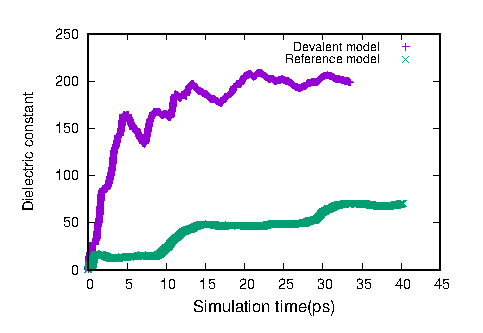
\includegraphics[width=0.45\textwidth]{dielectric}
\caption{Computed dielectric constant of the reference and devalent models as a function of simulation time.}\label{Fig:dielectric}
\end{figure} 

%RZK RW2 The statistical errors in dielectric constants are estimated to be 70±3, 180±5 for realistic and devalent models, respectively. This uncertainty is calculated from the fluctuations in the dielectric constant during the last 10 ps. It is not uncommon that relatively short trajectories can be sufficient to evaluate the dielectric constant. For example, R. Car et al. [Phys. Rev. Lett. 2007, 98, 247401] used a 20 ps simulation with PBE functional to compute the dielectric constant of water.

\section{Self-diffusion coefficient and shear viscosity} 

\begin{figure}[t]
\includegraphics[width=0.45\textwidth]{msd}
\caption{Diffusion constant as a function of the system size, for 64, 125 and 256 water molecules. 
The square dots are from simulation and the solid line is a linear fit.}\label{Fig:dfs}
\end{figure} 

The diffusion constant for a periodic system is known to have strong dependence on the size of the simulation box $L$, due to the long-range drag exerted on a particle by its periodic images~\cite{dunweg1993molecular}. 
Fortunately, the diffusion constant in the infinitely large simulation box $D(\infty)$ can be estimated from several finite-size simulations using the following well-known relation~\cite{dunweg1993molecular}:
%
\bea
D(\infty) = D(L) + \frac{k_BT\zeta}{6\pi \eta L},
\eea
%
where $D(L)$ is the diffusion constant for a system of size $L$, $\eta$ is the translational shear viscosity, and $\zeta$ is a constant of 2.837. 
We calculated the diffusion constant $D(\infty)$ using least squares fitting to the data obtained for systems of 64, 125, and 256 molecules (Figure~\ref{Fig:dfs}). The viscosity is obtained via the slope of the $D(L)$ dependence on $1/L$.

\section{HB lifetime} 

The continuous HB time-correlation function $C_{\text{HB}}(\tau)$ is defined as 
%
\bea
C_{\text{HB}}(\tau) = \frac{\sum_{ij}\langle \theta_{ij}(\tau)\theta_{ij}(0) \rangle}{\sum_{ij}\langle \theta_{ij}(0) \theta_{ij}(0) \rangle} \label{Eq:HBdecay},
\eea
%
where the HB survival function $\theta_{ij}(\tau)$ is equal to 1 if there is a HB formed between molecules $i$ and $j$ \emph{throughout} the time period from $t=0$ to $t=\tau$ and is otherwise equal to zero~\cite{rapaport1983hydrogen,starr1999fast}. 
In the long-time limit, the time-correlation function decays exponentially as shown in Figure~\ref{Fig:HBdecay}. 
The HB lifetime is defined as the rate of its decay $C_{\text{HB}}(\tau) \sim e^{-\tau/\tau_{\text{HB}}}$ and is computed as the slope of the logarithm of $C_{\text{HB}}(\tau)$.


\begin{figure}
\includegraphics[width=0.45\textwidth]{new_hbdecay}
\caption{HB time autocorrelation function for the reference and devalent systems.} \label{Fig:HBdecay}
\end{figure}

\section{Basis set dependence of the results} 

\begin{figure}
\includegraphics[width=0.45\textwidth]{basis_ir}
\includegraphics[width=0.45\textwidth]{basis_rdf}
\caption{IR spectra and oxygen-oxygen radial distribution functions calculated with TZV2P and aug-TZV2P basis sets.}\label{Fig:basis}
\end{figure} 

As indicated in the Computational Methods section, the accurate separation of donor-acceptor interactions from polarization effects is verified by performing simulations with two Gaussian basis sets of different sizes. 
To make the test stringent, the TZV2P basis set was extended by adding a set of diffuse functions with small exponents. 
The results of both simulations shown in Figure~\ref{Fig:basis} are practically identical. 
This indicates that TZV2P results are sufficiently stable with respect to a moderate increase in the basis set size. 
For larger basis sets, the role of intermolecular covalency will be spuriously decreased.


\fi % maintext - SI switch

\begin{thebibliography}{10}
\expandafter\ifx\csname url\endcsname\relax
  \def\url#1{\texttt{#1}}\fi
\expandafter\ifx\csname urlprefix\endcsname\relax\def\urlprefix{URL }\fi
\providecommand{\bibinfo}[2]{#2}
\providecommand{\eprint}[2][]{\url{#2}}

\bibitem{eisenberg2005structure}
\bibinfo{author}{Eisenberg, D.} \& \bibinfo{author}{Kauzmann, W.}
\newblock \emph{\bibinfo{title}{The structure and properties of water}}
  (\bibinfo{publisher}{Oxford University Press on Demand},
  \bibinfo{year}{2005}).

\bibitem{lee2011effects}
\bibinfo{author}{Lee, A.~J.} \& \bibinfo{author}{Rick, S.~W.}
\newblock \bibinfo{title}{The effects of charge transfer on the properties of
  liquid water}.
\newblock \emph{\bibinfo{journal}{J. Chem. Phys.}}
  \textbf{\bibinfo{volume}{134}}, \bibinfo{pages}{184507}
  (\bibinfo{year}{2011}).

\bibitem{gordon2013accurate}
\bibinfo{author}{Gordon, M.~S.}, \bibinfo{author}{Smith, Q.~A.},
  \bibinfo{author}{Xu, P.} \& \bibinfo{author}{Slipchenko, L.~V.}
\newblock \bibinfo{title}{Accurate first principles model potentials for
  intermolecular interactions}.
\newblock \emph{\bibinfo{journal}{Annu. Rev. Phys. Chem.}}
  \textbf{\bibinfo{volume}{64}}, \bibinfo{pages}{553--578}
  (\bibinfo{year}{2013}).

\bibitem{stevens1987frozen}
\bibinfo{author}{Stevens, W.~J.} \& \bibinfo{author}{Fink, W.~H.}
\newblock \bibinfo{title}{Frozen fragment reduced variational space analysis of
  hydrogen bonding interactions. application to the water dimer}.
\newblock \emph{\bibinfo{journal}{Chem. Phys. Lett.}}
  \textbf{\bibinfo{volume}{139}}, \bibinfo{pages}{15--22}
  (\bibinfo{year}{1987}).

\bibitem{stone1993computation}
\bibinfo{author}{Stone, A.~J.}
\newblock \bibinfo{title}{Computation of charge-transfer energies by
  perturbation theory}.
\newblock \emph{\bibinfo{journal}{Chem. Phys. Lett.}}
  \textbf{\bibinfo{volume}{211}}, \bibinfo{pages}{101--109}
  (\bibinfo{year}{1993}).

\bibitem{chen1996energy}
\bibinfo{author}{Chen, W.} \& \bibinfo{author}{Gordon, M.~S.}
\newblock \bibinfo{title}{Energy decomposition analyses for many-body
  interaction and applications to water complexes}.
\newblock \emph{\bibinfo{journal}{J. Phys. Chem}}
  \textbf{\bibinfo{volume}{100}}, \bibinfo{pages}{14316--14328}
  (\bibinfo{year}{1996}).

\bibitem{schenter1996natural}
\bibinfo{author}{Schenter, G.~K.} \& \bibinfo{author}{Glendening, E.~D.}
\newblock \bibinfo{title}{Natural energy decomposition analysis: The linear
  response electrical self energy}.
\newblock \emph{\bibinfo{journal}{J. Phys. Chem}}
  \textbf{\bibinfo{volume}{100}}, \bibinfo{pages}{17152--17156}
  (\bibinfo{year}{1996}).

\bibitem{glendening2005natural}
\bibinfo{author}{Glendening, E.~D.}
\newblock \bibinfo{title}{Natural energy decomposition analysis: Extension to
  density functional methods and analysis of cooperative effects in water
  clusters}.
\newblock \emph{\bibinfo{journal}{J. Phys. Chem. A}}
  \textbf{\bibinfo{volume}{109}}, \bibinfo{pages}{11936--11940}
  (\bibinfo{year}{2005}).

\bibitem{weinhold2005resonance}
\bibinfo{author}{Weinhold, F.}
\newblock \bibinfo{title}{Resonance character of hydrogen-bonding interactions
  in water and other h-bonded species}.
\newblock \emph{\bibinfo{journal}{Adv. Protein Chem.}}
  \textbf{\bibinfo{volume}{72}}, \bibinfo{pages}{121--155}
  (\bibinfo{year}{2005}).

\bibitem{piquemal2005csov}
\bibinfo{author}{Piquemal, J.-P.}, \bibinfo{author}{Marquez, A.},
  \bibinfo{author}{Parisel, O.} \& \bibinfo{author}{Giessner-Prettre, C.}
\newblock \bibinfo{title}{A csov study of the difference between hf and dft
  intermolecular interaction energy values: The importance of the charge
  transfer contribution}.
\newblock \emph{\bibinfo{journal}{J. Comput. Chem.}}
  \textbf{\bibinfo{volume}{26}}, \bibinfo{pages}{1052--1062}
  (\bibinfo{year}{2005}).

\bibitem{khaliullin2009electron}
\bibinfo{author}{Khaliullin, R.~Z.}, \bibinfo{author}{Bell, A.~T.} \&
  \bibinfo{author}{Head-Gordon, M.}
\newblock \bibinfo{title}{Electron donation in the water--water hydrogen bond}.
\newblock \emph{\bibinfo{journal}{Chem. Eur. J.}}
  \textbf{\bibinfo{volume}{15}}, \bibinfo{pages}{851--855}
  (\bibinfo{year}{2009}).

\bibitem{cobar2012examination}
\bibinfo{author}{Cobar, E.~A.}, \bibinfo{author}{Horn, P.~R.},
  \bibinfo{author}{Bergman, R.~G.} \& \bibinfo{author}{Head-Gordon, M.}
\newblock \bibinfo{title}{Examination of the hydrogen-bonding networks in small
  water clusters (n= 2--5, 13, 17) using absolutely localized molecular orbital
  energy decomposition analysis}.
\newblock \emph{\bibinfo{journal}{Phys. Chem. Chem. Phys.}}
  \textbf{\bibinfo{volume}{14}}, \bibinfo{pages}{15328--15339}
  (\bibinfo{year}{2012}).

\bibitem{guevara2016hydrogen}
\bibinfo{author}{Guevara-Vela, J.~M.} \emph{et~al.}
\newblock \bibinfo{title}{Hydrogen bond cooperativity and anticooperativity
  within the water hexamer}.
\newblock \emph{\bibinfo{journal}{Phys. Chem. Chem. Phys.}}
  \textbf{\bibinfo{volume}{18}}, \bibinfo{pages}{19557--19566}
  (\bibinfo{year}{2016}).

\bibitem{isaacs1999covalency}
\bibinfo{author}{Isaacs, E.} \emph{et~al.}
\newblock \bibinfo{title}{Covalency of the hydrogen bond in ice: A direct x-ray
  measurement}.
\newblock \emph{\bibinfo{journal}{Phys. Rev. Lett.}}
  \textbf{\bibinfo{volume}{82}}, \bibinfo{pages}{600} (\bibinfo{year}{1999}).

\bibitem{ghanty2000hydrogen}
\bibinfo{author}{Ghanty, T.~K.}, \bibinfo{author}{Staroverov, V.~N.},
  \bibinfo{author}{Koren, P.~R.} \& \bibinfo{author}{Davidson, E.~R.}
\newblock \bibinfo{title}{Is the hydrogen bond in water dimer and ice
  covalent?}
\newblock \emph{\bibinfo{journal}{J. Am. Chem. Soc.}}
  \textbf{\bibinfo{volume}{122}}, \bibinfo{pages}{1210--1214}
  (\bibinfo{year}{2000}).

\bibitem{stone2017natural}
\bibinfo{author}{Stone, A.~J.}
\newblock \bibinfo{title}{Natural bond orbitals and the nature of the hydrogen
  bond}.
\newblock \emph{\bibinfo{journal}{J. Phys. Chem. A}}
  \textbf{\bibinfo{volume}{121}}, \bibinfo{pages}{1531--1534}
  (\bibinfo{year}{2017}).

\bibitem{weinhold1998natural}
\bibinfo{author}{Weinhold, F.}
\newblock \bibinfo{title}{Natural bond orbital methods}.
\newblock \emph{\bibinfo{journal}{Encyclopedia of computational chemistry}}
  (\bibinfo{year}{1998}).

\bibitem{glendening1994natural}
\bibinfo{author}{Glendening, E.~D.} \& \bibinfo{author}{Streitwieser, A.}
\newblock \bibinfo{title}{Natural energy decomposition analysis: An energy
  partitioning procedure for molecular interactions with application to weak
  hydrogen bonding, strong ionic, and moderate donor--acceptor interactions}.
\newblock \emph{\bibinfo{journal}{J. Chem. Phys.}}
  \textbf{\bibinfo{volume}{100}}, \bibinfo{pages}{2900--2909}
  (\bibinfo{year}{1994}).

\bibitem{kitaura1976new}
\bibinfo{author}{Kitaura, K.} \& \bibinfo{author}{Morokuma, K.}
\newblock \bibinfo{title}{A new energy decomposition scheme for molecular
  interactions within the hartree-fock approximation}.
\newblock \emph{\bibinfo{journal}{Int. J. Quantum Chem.}}
  \textbf{\bibinfo{volume}{10}}, \bibinfo{pages}{325--340}
  (\bibinfo{year}{1976}).

\bibitem{bagus1984new}
\bibinfo{author}{Bagus, P.~S.}, \bibinfo{author}{Hermann, K.} \&
  \bibinfo{author}{Bauschlicher~Jr, C.~W.}
\newblock \bibinfo{title}{A new analysis of charge transfer and polarization
  for ligand--metal bonding: Model studies of al4co and al4nh3}.
\newblock \emph{\bibinfo{journal}{J. Chem. Phys.}}
  \textbf{\bibinfo{volume}{80}}, \bibinfo{pages}{4378--4386}
  (\bibinfo{year}{1984}).

\bibitem{bagus1992decomposition}
\bibinfo{author}{Bagus, P.~S.} \& \bibinfo{author}{Illas, F.}
\newblock \bibinfo{title}{Decomposition of the chemisorption bond by
  constrained variations: order of the variations and construction of the
  variational spaces}.
\newblock \emph{\bibinfo{journal}{J. Chem. Phys.}}
  \textbf{\bibinfo{volume}{96}}, \bibinfo{pages}{8962--8970}
  (\bibinfo{year}{1992}).

\bibitem{mo2000energy}
\bibinfo{author}{Mo, Y.}, \bibinfo{author}{Gao, J.} \&
  \bibinfo{author}{Peyerimhoff, S.~D.}
\newblock \bibinfo{title}{Energy decomposition analysis of intermolecular
  interactions using a block-localized wave function approach}.
\newblock \emph{\bibinfo{journal}{J. Chem. Phys.}}
  \textbf{\bibinfo{volume}{112}}, \bibinfo{pages}{5530--5538}
  (\bibinfo{year}{2000}).

\bibitem{misquitta2013charge}
\bibinfo{author}{Misquitta, A.~J.}
\newblock \bibinfo{title}{Charge transfer from regularized symmetry-adapted
  perturbation theory}.
\newblock \emph{\bibinfo{journal}{J. Chem. Theory Comput.}}
  \textbf{\bibinfo{volume}{9}}, \bibinfo{pages}{5313--5326}
  (\bibinfo{year}{2013}).

\bibitem{khaliullin2007unravelling}
\bibinfo{author}{Khaliullin, R.~Z.}, \bibinfo{author}{Cobar, E.~A.},
  \bibinfo{author}{Lochan, R.~C.}, \bibinfo{author}{Bell, A.~T.} \&
  \bibinfo{author}{Head-Gordon, M.}
\newblock \bibinfo{title}{Unravelling the origin of intermolecular interactions
  using absolutely localized molecular orbitals}.
\newblock \emph{\bibinfo{journal}{J. Phys. Chem. A}}
  \textbf{\bibinfo{volume}{111}}, \bibinfo{pages}{8753--8765}
  (\bibinfo{year}{2007}).

\bibitem{fransson2016x}
\bibinfo{author}{Fransson, T.} \emph{et~al.}
\newblock \bibinfo{title}{X-ray and electron spectroscopy of water}.
\newblock \emph{\bibinfo{journal}{Chem. Rev.}} \textbf{\bibinfo{volume}{116}},
  \bibinfo{pages}{7551--7569} (\bibinfo{year}{2016}).

\bibitem{NatureComm2013}
\bibinfo{author}{K{\"u}hne, T.~D.} \& \bibinfo{author}{Khaliullin, R.~Z.}
\newblock \bibinfo{title}{Electronic signature of the instantaneous asymmetry
  in the first coordination shell of liquid water}.
\newblock \emph{\bibinfo{journal}{Nat. Commun.}} \textbf{\bibinfo{volume}{4}},
  \bibinfo{pages}{1450} (\bibinfo{year}{2013}).

\bibitem{JPCL2013}
\bibinfo{author}{Zhang, C.}, \bibinfo{author}{Khaliullin, R.~Z.},
  \bibinfo{author}{Bovi, D.}, \bibinfo{author}{Guidoni, L.} \&
  \bibinfo{author}{K{\"u}hne, T.~D.}
\newblock \bibinfo{title}{Vibrational signature of water molecules in
  asymmetric hydrogen bonding environments}.
\newblock \emph{\bibinfo{journal}{J. Phys. Chem. Lett.}}
  \textbf{\bibinfo{volume}{4}}, \bibinfo{pages}{3245--3250}
  (\bibinfo{year}{2013}).

\bibitem{Faraday2011}
\bibinfo{author}{Ramos-Cordoba, E.}, \bibinfo{author}{Lambrecht, D.~S.} \&
  \bibinfo{author}{Head-Gordon, M.}
\newblock \bibinfo{title}{Charge-transfer and the hydrogen bond: Spectroscopic
  and structural implications from electronic structure calculations}.
\newblock \emph{\bibinfo{journal}{Faraday Discuss.}}
  \textbf{\bibinfo{volume}{150}}, \bibinfo{pages}{345--362}
  (\bibinfo{year}{2011}).

\bibitem{lenz2006theoretical}
\bibinfo{author}{Lenz, A.} \& \bibinfo{author}{Ojam{\"a}e, L.}
\newblock \bibinfo{title}{Theoretical ir spectra for water clusters (h2o) n (n=
  6- 22, 28, 30) and identification of spectral contributions from different
  h-bond conformations in gaseous and liquid water}.
\newblock \emph{\bibinfo{journal}{J. Phys. Chem. A}}
  \textbf{\bibinfo{volume}{110}}, \bibinfo{pages}{13388--13393}
  (\bibinfo{year}{2006}).

\bibitem{NatureComm2015}
\bibinfo{author}{Elgabarty, H.}, \bibinfo{author}{Khaliullin, R.~Z.} \&
  \bibinfo{author}{K{\"u}hne, T.~D.}
\newblock \bibinfo{title}{Covalency of hydrogen bonds in liquid water can be
  probed by proton nuclear magnetic resonance experiments}.
\newblock \emph{\bibinfo{journal}{Nat. Commun.}} \textbf{\bibinfo{volume}{6}}
  (\bibinfo{year}{2015}).

\bibitem{Khaliullin2013JCTC}
\bibinfo{author}{Khaliullin, R.~Z.}, \bibinfo{author}{VandeVondele, J.} \&
  \bibinfo{author}{Hutter, J.}
\newblock \bibinfo{title}{Efficient linear-scaling density functional theory
  for molecular systems}.
\newblock \emph{\bibinfo{journal}{J. Chem. Theory Comput.}}
  \textbf{\bibinfo{volume}{9}}, \bibinfo{pages}{4421--4427}
  (\bibinfo{year}{2013}).

\bibitem{khaliullin2006efficient}
\bibinfo{author}{Khaliullin, R.~Z.}, \bibinfo{author}{Head-Gordon, M.} \&
  \bibinfo{author}{Bell, A.~T.}
\newblock \bibinfo{title}{An efficient self-consistent field method for large
  systems of weakly interacting components}.
\newblock \emph{\bibinfo{journal}{J. Chem. Phys.}}
  \textbf{\bibinfo{volume}{124}}, \bibinfo{pages}{204105}
  (\bibinfo{year}{2006}).

\bibitem{stoll1980use}
\bibinfo{author}{Stoll, H.}, \bibinfo{author}{Wagenblast, G.} \&
  \bibinfo{author}{Preu$\beta$, H.}
\newblock \bibinfo{title}{On the use of local basis sets for localized
  molecular orbitals}.
\newblock \emph{\bibinfo{journal}{Theor. Chem. Acc.}}
  \textbf{\bibinfo{volume}{57}}, \bibinfo{pages}{169--178}
  (\bibinfo{year}{1980}).

\bibitem{grimme2010consistent}
\bibinfo{author}{Grimme, S.}, \bibinfo{author}{Antony, J.},
  \bibinfo{author}{Ehrlich, S.} \& \bibinfo{author}{Krieg, H.}
\newblock \bibinfo{title}{A consistent and accurate ab initio parametrization
  of density functional dispersion correction (dft-d) for the 94 elements
  h-pu}.
\newblock \emph{\bibinfo{journal}{J. Chem. Phys.}}
  \textbf{\bibinfo{volume}{132}}, \bibinfo{pages}{154104}
  (\bibinfo{year}{2010}).

\bibitem{becke1988density}
\bibinfo{author}{Becke, A.~D.}
\newblock \bibinfo{title}{Density-functional exchange-energy approximation with
  correct asymptotic behavior}.
\newblock \emph{\bibinfo{journal}{Phys. Rev. A}} \textbf{\bibinfo{volume}{38}},
  \bibinfo{pages}{3098} (\bibinfo{year}{1988}).

\bibitem{lee1988development}
\bibinfo{author}{Lee, C.}, \bibinfo{author}{Yang, W.} \& \bibinfo{author}{Parr,
  R.~G.}
\newblock \bibinfo{title}{Development of the colle-salvetti correlation-energy
  formula into a functional of the electron density}.
\newblock \emph{\bibinfo{journal}{Phys. Rev. B}} \textbf{\bibinfo{volume}{37}},
  \bibinfo{pages}{785} (\bibinfo{year}{1988}).

\bibitem{vandevondele2007gaussian}
\bibinfo{author}{VandeVondele, J.} \& \bibinfo{author}{Hutter, J.}
\newblock \bibinfo{title}{Gaussian basis sets for accurate calculations on
  molecular systems in gas and condensed phases}.
\newblock \emph{\bibinfo{journal}{J. Chem. Phys.}}
  \textbf{\bibinfo{volume}{127}}, \bibinfo{pages}{114105}
  (\bibinfo{year}{2007}).

\bibitem{cheng2012alignment}
\bibinfo{author}{Cheng, J.} \& \bibinfo{author}{Sprik, M.}
\newblock \bibinfo{title}{Alignment of electronic energy levels at
  electrochemical interfaces}.
\newblock \emph{\bibinfo{journal}{Phys. Chem. Chem. Phys.}}
  \textbf{\bibinfo{volume}{14}}, \bibinfo{pages}{11245--11267}
  (\bibinfo{year}{2012}).

\bibitem{chen2017ab}
\bibinfo{author}{Chen, M.} \emph{et~al.}
\newblock \bibinfo{title}{Ab initio theory and modeling of water}.
\newblock \emph{\bibinfo{journal}{Proc. Natl. Acad. Sci. U.S.A.}}
  \textbf{\bibinfo{volume}{114}}, \bibinfo{pages}{10846--10851}
  (\bibinfo{year}{2017}).

\bibitem{adriaanse2012aqueous}
\bibinfo{author}{Adriaanse, C.} \emph{et~al.}
\newblock \bibinfo{title}{Aqueous redox chemistry and the electronic band
  structure of liquid water}.
\newblock \emph{\bibinfo{journal}{J. Phys. Chem. A}}
  \textbf{\bibinfo{volume}{3}}, \bibinfo{pages}{3411--3415}
  (\bibinfo{year}{2012}).

\bibitem{gillan2016perspective}
\bibinfo{author}{Gillan, M.~J.}, \bibinfo{author}{Alf{\`e}, D.} \&
  \bibinfo{author}{Michaelides, A.}
\newblock \bibinfo{title}{Perspective: How good is dft for water?}
\newblock \emph{\bibinfo{journal}{J. Chem. Phys.}}
  \textbf{\bibinfo{volume}{144}}, \bibinfo{pages}{130901}
  (\bibinfo{year}{2016}).

\bibitem{ma2012ab}
\bibinfo{author}{Ma, Z.}, \bibinfo{author}{Zhang, Y.} \&
  \bibinfo{author}{Tuckerman, M.~E.}
\newblock \bibinfo{title}{Ab initio molecular dynamics study of water at
  constant pressure using converged basis sets and empirical dispersion
  corrections}.
\newblock \emph{\bibinfo{journal}{J. Chem. Phys.}}
  \textbf{\bibinfo{volume}{137}}, \bibinfo{pages}{044506}
  (\bibinfo{year}{2012}).

\bibitem{bankura2014structure}
\bibinfo{author}{Bankura, A.}, \bibinfo{author}{Karmakar, A.},
  \bibinfo{author}{Carnevale, V.}, \bibinfo{author}{Chandra, A.} \&
  \bibinfo{author}{Klein, M.~L.}
\newblock \bibinfo{title}{Structure, dynamics, and spectral diffusion of water
  from first-principles molecular dynamics}.
\newblock \emph{\bibinfo{journal}{J. Phys. Chem.C}}
  \textbf{\bibinfo{volume}{118}}, \bibinfo{pages}{29401--29411}
  (\bibinfo{year}{2014}).

\bibitem{khaliullin2013microscopic}
\bibinfo{author}{Khaliullin, R.~Z.} \& \bibinfo{author}{K{\"u}hne, T.~D.}
\newblock \bibinfo{title}{Microscopic properties of liquid water from combined
  ab initio molecular dynamics and energy decomposition studies}.
\newblock \emph{\bibinfo{journal}{Phys. Chem. Chem. Phys.}}
  \textbf{\bibinfo{volume}{15}}, \bibinfo{pages}{15746--15766}
  (\bibinfo{year}{2013}).

\bibitem{lee2007dynamical}
\bibinfo{author}{Lee, H.-S.} \& \bibinfo{author}{Tuckerman, M.~E.}
\newblock \bibinfo{title}{Dynamical properties of liquid water from ab initio
  molecular dynamics performed in the complete basis set limit}.
\newblock \emph{\bibinfo{journal}{J. Chem. Phys.}}
  \textbf{\bibinfo{volume}{126}}, \bibinfo{pages}{164501}
  (\bibinfo{year}{2007}).

\bibitem{schneider2016decomposition}
\bibinfo{author}{Schneider, W.~B.} \emph{et~al.}
\newblock \bibinfo{title}{Decomposition of intermolecular interaction energies
  within the local pair natural orbital coupled cluster framework}.
\newblock \emph{\bibinfo{journal}{J. Chem. Theory Comput.}}
  \textbf{\bibinfo{volume}{12}}, \bibinfo{pages}{4778--4792}
  (\bibinfo{year}{2016}).

\bibitem{azar2012energy}
\bibinfo{author}{Azar, R.~J.} \& \bibinfo{author}{Head-Gordon, M.}
\newblock \bibinfo{title}{An energy decomposition analysis for intermolecular
  interactions from an absolutely localized molecular orbital reference at the
  coupled-cluster singles and doubles level}.
\newblock \emph{\bibinfo{journal}{J. Chem. Phys.}}
  \textbf{\bibinfo{volume}{136}}, \bibinfo{pages}{024103}
  (\bibinfo{year}{2012}).

\bibitem{azar2015similarity}
\bibinfo{author}{Azar, R.~J.} \& \bibinfo{author}{Head-Gordon, M.}
\newblock \bibinfo{title}{Similarity-transformed perturbation theory on top of
  truncated local coupled cluster solutions: Theory and applications to
  intermolecular interactions}.
\newblock \emph{\bibinfo{journal}{J. Chem. Phys.}}
  \textbf{\bibinfo{volume}{142}}, \bibinfo{pages}{204101}
  (\bibinfo{year}{2015}).

\bibitem{kuhne2014nature}
\bibinfo{author}{K{\"u}hne, T.~D.} \& \bibinfo{author}{Khaliullin, R.~Z.}
\newblock \bibinfo{title}{Nature of the asymmetry in the hydrogen-bond networks
  of hexagonal ice and liquid water}.
\newblock \emph{\bibinfo{journal}{J. Am. Chem. Soc.}}
  \textbf{\bibinfo{volume}{136}}, \bibinfo{pages}{3395--3399}
  (\bibinfo{year}{2014}).

\bibitem{skinner2013benchmark}
\bibinfo{author}{Skinner, L.~B.} \emph{et~al.}
\newblock \bibinfo{title}{Benchmark oxygen-oxygen pair-distribution function of
  ambient water from x-ray diffraction measurements with a wide q-range}.
\newblock \emph{\bibinfo{journal}{J. Chem. Phys.}}
  \textbf{\bibinfo{volume}{138}}, \bibinfo{pages}{074506}
  (\bibinfo{year}{2013}).

\bibitem{modig2003temperature}
\bibinfo{author}{Modig, K.}, \bibinfo{author}{Pfrommer, B.~G.} \&
  \bibinfo{author}{Halle, B.}
\newblock \bibinfo{title}{Temperature-dependent hydrogen-bond geometry in
  liquid water}.
\newblock \emph{\bibinfo{journal}{Phys. Rev. Lett.}}
  \textbf{\bibinfo{volume}{90}}, \bibinfo{pages}{075502}
  (\bibinfo{year}{2003}).

\bibitem{arunan2011definition}
\bibinfo{author}{Arunan, E.} \emph{et~al.}
\newblock \bibinfo{title}{Definition of the hydrogen bond (iupac
  recommendations 2011)}.
\newblock \emph{\bibinfo{journal}{Pure Appl. Chem.}}
  \textbf{\bibinfo{volume}{83}}, \bibinfo{pages}{1637--1641}
  (\bibinfo{year}{2011}).

\bibitem{TIP3P}
\bibinfo{author}{Mahoney, M.~W.} \& \bibinfo{author}{Jorgensen, W.~L.}
\newblock \bibinfo{title}{A five-site model for liquid water and the
  reproduction of the density anomaly by rigid, nonpolarizable potential
  functions}.
\newblock \emph{\bibinfo{journal}{J. Chem. Phys.}}
  \textbf{\bibinfo{volume}{112}}, \bibinfo{pages}{8910--8922}
  (\bibinfo{year}{2000}).

\bibitem{rey2002hydrogen}
\bibinfo{author}{Rey, R.}, \bibinfo{author}{M{\o}ller, K.~B.} \&
  \bibinfo{author}{Hynes, J.~T.}
\newblock \bibinfo{title}{Hydrogen bond dynamics in water and ultrafast
  infrared spectroscopy}.
\newblock \emph{\bibinfo{journal}{J. Phys. Chem. A}}
  \textbf{\bibinfo{volume}{106}}, \bibinfo{pages}{11993--11996}
  (\bibinfo{year}{2002}).

\bibitem{lawrence2003vibrational}
\bibinfo{author}{Lawrence, C.} \& \bibinfo{author}{Skinner, J.}
\newblock \bibinfo{title}{Vibrational spectroscopy of hod in liquid d 2 o. iii.
  spectral diffusion, and hydrogen-bonding and rotational dynamics}.
\newblock \emph{\bibinfo{journal}{J. Chem. Phys.}}
  \textbf{\bibinfo{volume}{118}}, \bibinfo{pages}{264--272}
  (\bibinfo{year}{2003}).

\bibitem{thomas2013computing}
\bibinfo{author}{Thomas, M.}, \bibinfo{author}{Brehm, M.},
  \bibinfo{author}{Fligg, R.}, \bibinfo{author}{V{\"o}hringer, P.} \&
  \bibinfo{author}{Kirchner, B.}
\newblock \bibinfo{title}{Computing vibrational spectra from ab initio
  molecular dynamics}.
\newblock \emph{\bibinfo{journal}{Phys. Chem. Chem. Phys.}}
  \textbf{\bibinfo{volume}{15}}, \bibinfo{pages}{6608--6622}
  (\bibinfo{year}{2013}).

\bibitem{marsalek2017quantum}
\bibinfo{author}{Marsalek, O.} \& \bibinfo{author}{Markland, T.~E.}
\newblock \bibinfo{title}{Quantum dynamics and spectroscopy of ab initio liquid
  water: The interplay of nuclear and electronic quantum effects}.
\newblock \emph{\bibinfo{journal}{J. Phys. Chem. Lett.}}
  \textbf{\bibinfo{volume}{8}}, \bibinfo{pages}{1545--1551}
  (\bibinfo{year}{2017}).

\bibitem{medders2015infrared}
\bibinfo{author}{Medders, G.~R.} \& \bibinfo{author}{Paesani, F.}
\newblock \bibinfo{title}{Infrared and raman spectroscopy of liquid water
  through “first-principles” many-body molecular dynamics}.
\newblock \emph{\bibinfo{journal}{J. Chem. Theory Comput.}}
  \textbf{\bibinfo{volume}{11}}, \bibinfo{pages}{1145--1154}
  (\bibinfo{year}{2015}).

\bibitem{joseph2007red}
\bibinfo{author}{Joseph, J.} \& \bibinfo{author}{Jemmis, E.~D.}
\newblock \bibinfo{title}{Red-, blue-, or no-shift in hydrogen bonds: a unified
  explanation}.
\newblock \emph{\bibinfo{journal}{J. Am. Chem. Soc.}}
  \textbf{\bibinfo{volume}{129}}, \bibinfo{pages}{4620--4632}
  (\bibinfo{year}{2007}).

\bibitem{iogansen1999direct}
\bibinfo{author}{Iogansen, A.}
\newblock \bibinfo{title}{Direct proportionality of the hydrogen bonding energy
  and the intensification of the stretching $\nu$ (xh) vibration in infrared
  spectra}.
\newblock \emph{\bibinfo{journal}{Spectrochim. Acta A}}
  \textbf{\bibinfo{volume}{55}}, \bibinfo{pages}{1585--1612}
  (\bibinfo{year}{1999}).

\bibitem{marechal2006hydrogen}
\bibinfo{author}{Mar{\'e}chal, Y.}
\newblock \emph{\bibinfo{title}{The hydrogen bond and the water molecule: The
  physics and chemistry of water, aqueous and bio-media}}
  (\bibinfo{publisher}{Elsevier}, \bibinfo{year}{2006}).

\bibitem{marzari1997maximally}
\bibinfo{author}{Marzari, N.} \& \bibinfo{author}{Vanderbilt, D.}
\newblock \bibinfo{title}{Maximally localized generalized wannier functions for
  composite energy bands}.
\newblock \emph{\bibinfo{journal}{Phys. Rev. B}} \textbf{\bibinfo{volume}{56}},
  \bibinfo{pages}{12847} (\bibinfo{year}{1997}).

\bibitem{sharma2007dipolar}
\bibinfo{author}{Sharma, M.}, \bibinfo{author}{Resta, R.} \&
  \bibinfo{author}{Car, R.}
\newblock \bibinfo{title}{Dipolar correlations and the dielectric permittivity
  of water}.
\newblock \emph{\bibinfo{journal}{Phys. Rev. Lett.}}
  \textbf{\bibinfo{volume}{98}}, \bibinfo{pages}{247401}
  (\bibinfo{year}{2007}).

\bibitem{badyal2000electron}
\bibinfo{author}{Badyal, Y.} \emph{et~al.}
\newblock \bibinfo{title}{Electron distribution in water}.
\newblock \emph{\bibinfo{journal}{J. Chem. Phys.}}
  \textbf{\bibinfo{volume}{112}}, \bibinfo{pages}{9206--9208}
  (\bibinfo{year}{2000}).

\bibitem{haynes2014crc}
\bibinfo{author}{Haynes, W.~M.}
\newblock \emph{\bibinfo{title}{CRC handbook of chemistry and physics}}
  (\bibinfo{publisher}{CRC press}, \bibinfo{year}{2014}).

\bibitem{lawrence2003ultrafast}
\bibinfo{author}{Lawrence, C.} \& \bibinfo{author}{Skinner, J.}
\newblock \bibinfo{title}{Ultrafast infrared spectroscopy probes
  hydrogen-bonding dynamics in liquid water}.
\newblock \emph{\bibinfo{journal}{Chem. Phys. Lett.}}
  \textbf{\bibinfo{volume}{369}}, \bibinfo{pages}{472--477}
  (\bibinfo{year}{2003}).

\bibitem{marti1996molecular}
\bibinfo{author}{Marti, J.}, \bibinfo{author}{Padro, J.} \&
  \bibinfo{author}{Guardia, E.}
\newblock \bibinfo{title}{Molecular dynamics simulation of liquid water along
  the coexistence curve: Hydrogen bonds and vibrational spectra}.
\newblock \emph{\bibinfo{journal}{J. Chem. Phys.}}
  \textbf{\bibinfo{volume}{105}}, \bibinfo{pages}{639--649}
  (\bibinfo{year}{1996}).

\bibitem{starr1999fast}
\bibinfo{author}{Starr, F.~W.}, \bibinfo{author}{Nielsen, J.~K.} \&
  \bibinfo{author}{Stanley, H.~E.}
\newblock \bibinfo{title}{Fast and slow dynamics of hydrogen bonds in liquid
  water}.
\newblock \emph{\bibinfo{journal}{Phys. Rev. Lett.}}
  \textbf{\bibinfo{volume}{82}}, \bibinfo{pages}{2294} (\bibinfo{year}{1999}).

\bibitem{dunweg1993molecular}
\bibinfo{author}{D{\"u}nweg, B.} \& \bibinfo{author}{Kremer, K.}
\newblock \bibinfo{title}{Molecular dynamics simulation of a polymer chain in
  solution}.
\newblock \emph{\bibinfo{journal}{J. Chem. Phys.}}
  \textbf{\bibinfo{volume}{99}}, \bibinfo{pages}{6983--6997}
  (\bibinfo{year}{1993}).

\bibitem{hardy2001isotope}
\bibinfo{author}{Hardy, E.~H.}, \bibinfo{author}{Zygar, A.},
  \bibinfo{author}{Zeidler, M.~D.}, \bibinfo{author}{Holz, M.} \&
  \bibinfo{author}{Sacher, F.~D.}
\newblock \bibinfo{title}{Isotope effect on the translational and rotational
  motion in liquid water and ammonia}.
\newblock \emph{\bibinfo{journal}{J. Chem. Phys.}}
  \textbf{\bibinfo{volume}{114}}, \bibinfo{pages}{3174--3181}
  (\bibinfo{year}{2001}).

\bibitem{harris2004temperature}
\bibinfo{author}{Harris, K.~R.} \& \bibinfo{author}{Woolf, L.~A.}
\newblock \bibinfo{title}{Temperature and volume dependence of the viscosity of
  water and heavy water at low temperatures}.
\newblock \emph{\bibinfo{journal}{J. Chem. Eng. Data}}
  \textbf{\bibinfo{volume}{49}}, \bibinfo{pages}{1064--1069}
  (\bibinfo{year}{2004}).

\bibitem{rick2016polarizable}
\bibinfo{author}{Rick, S.~W.}
\newblock \bibinfo{title}{A polarizable, charge transfer model of water using
  the drude oscillator}.
\newblock \emph{\bibinfo{journal}{J. Comput. Chem.}}
  \textbf{\bibinfo{volume}{37}}, \bibinfo{pages}{2060--2066}
  (\bibinfo{year}{2016}).

\bibitem{vega2011simulating}
\bibinfo{author}{Vega, C.} \& \bibinfo{author}{Abascal, J.~L.}
\newblock \bibinfo{title}{Simulating water with rigid non-polarizable models: a
  general perspective}.
\newblock \emph{\bibinfo{journal}{Phys. Chem. Chem. Phys.}}
  \textbf{\bibinfo{volume}{13}}, \bibinfo{pages}{19663--19688}
  (\bibinfo{year}{2011}).

\bibitem{www:cp2k}
\bibinfo{title}{Cp2k open source molecular dynamics}.
\newblock \urlprefix\url{http://www.cp2k.org}.

\bibitem{hutter2014cp2k}
\bibinfo{author}{Hutter, J.}, \bibinfo{author}{Iannuzzi, M.},
  \bibinfo{author}{Schiffmann, F.} \& \bibinfo{author}{VandeVondele, J.}
\newblock \bibinfo{title}{Cp2k: atomistic simulations of condensed matter
  systems}.
\newblock \emph{\bibinfo{journal}{Wiley Interdisciplinary Reviews:
  Computational Molecular Science}} \textbf{\bibinfo{volume}{4}},
  \bibinfo{pages}{15--25} (\bibinfo{year}{2014}).

\bibitem{goedecker1996separable}
\bibinfo{author}{Goedecker, S.}, \bibinfo{author}{Teter, M.} \&
  \bibinfo{author}{Hutter, J.}
\newblock \bibinfo{title}{Separable dual-space gaussian pseudopotentials}.
\newblock \emph{\bibinfo{journal}{Phys. Rev. B}} \textbf{\bibinfo{volume}{54}},
  \bibinfo{pages}{1703} (\bibinfo{year}{1996}).

\bibitem{krack2005pseudopotentials}
\bibinfo{author}{Krack, M.}
\newblock \bibinfo{title}{Pseudopotentials for h to kr optimized for
  gradient-corrected exchange-correlation functionals}.
\newblock \emph{\bibinfo{journal}{Theor. Chem. Acc.}}
  \textbf{\bibinfo{volume}{114}}, \bibinfo{pages}{145--152}
  (\bibinfo{year}{2005}).

\bibitem{bussi2007canonical}
\bibinfo{author}{Bussi, G.}, \bibinfo{author}{Donadio, D.} \&
  \bibinfo{author}{Parrinello, M.}
\newblock \bibinfo{title}{Canonical sampling through velocity rescaling}.
\newblock \emph{\bibinfo{journal}{J. Chem. Phys.}}
  \textbf{\bibinfo{volume}{126}}, \bibinfo{pages}{014101}
  (\bibinfo{year}{2007}).

\bibitem{brehm2012travis}
\bibinfo{author}{Brehm, M.} \& \bibinfo{author}{Kirchner, B.}
\newblock \bibinfo{title}{Travis-a free analyzer and visualizer for monte carlo
  and molecular dynamics trajectories}.
\newblock \emph{\bibinfo{journal}{J. Cheminformatics}}
  \textbf{\bibinfo{volume}{4}}, \bibinfo{pages}{F1} (\bibinfo{year}{2012}).

\bibitem{horn2015polarization}
\bibinfo{author}{Horn, P.~R.} \& \bibinfo{author}{Head-Gordon, M.}
\newblock \bibinfo{title}{Polarization contributions to intermolecular
  interactions revisited with fragment electric-field response functions}.
\newblock \emph{\bibinfo{journal}{J. Chem. Phys.}}
  \textbf{\bibinfo{volume}{143}}, \bibinfo{pages}{114111}
  (\bibinfo{year}{2015}).

\bibitem{lao2016energy}
\bibinfo{author}{Lao, K.~U.} \& \bibinfo{author}{Herbert, J.~M.}
\newblock \bibinfo{title}{Energy decomposition analysis with a stable
  charge-transfer term for interpreting intermolecular interactions}.
\newblock \emph{\bibinfo{journal}{J. Chem. Theory Comput.}}
  \textbf{\bibinfo{volume}{12}}, \bibinfo{pages}{2569--2582}
  (\bibinfo{year}{2016}).

\end{thebibliography}
\end{document}
